\chapter{Tecniche di caratterizzazione dei workload}
I workload reali sono la migliore opzione per andare a valutare le performance specifiche di un dato sistema, il problema è che mantenere tale workload richiede un ingente quantità di memoria. Quindi è nata la necessità di trovare e ricercare delle tecniche che permettessero di poter caratterizzare un workload reale e ridurre la quantità di dati da memorizzare per poterne avere una statistica quanto meno affidabile

\section{Terminologia}
Gli argomenti che saranno affrontati durante tale capitolo richiedono una conoscenza della specifica terminologia utilizzata. In generale i concetti fondamentali da conoscere inerenti al dispositivo ed al componente da testare sono:
\begin{itemize}
    \item \textbf{DUT}(Device Under Test): Sistema che viene sottoposto ad uno specifico test (es. CPU o un processo di transazione)
    \item \textbf{CUT}(Component Under Test): Componente del sistema di cui si vogliono conoscere le performance (es.ALU o Unità Disco)
    \item \textbf{Metrica}: Metrica che si vuole andare a valutare per il CUT (es. MIPS o T/s)
\end{itemize}

\begin{figure}[h]
\centering
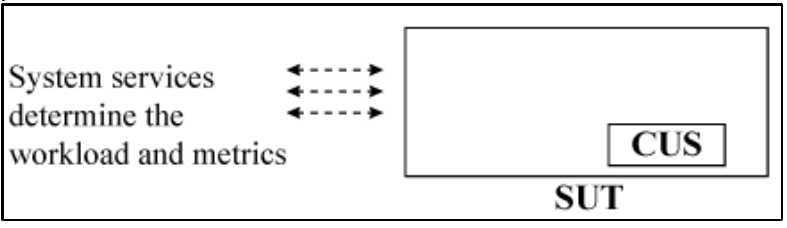
\includegraphics[width=.8\textwidth]{img/CUS-SUT.png}
\caption{Struttura del sistema di test}\label{img:cus-sut}
\end{figure}

Oltre la terminologia intrinseca al sistema di test bisogna definire anche la terminologia inerente ad altre entità interagenti. Quindi si definiscono i seguenti termini:
\begin{itemize}
    \item \textbf{User}: entità che esegue le richieste di servizio
    \item \textbf{Workload components}(Qualitative identifiers): Componenti basilari che mi permettono di capire a livello qualitativo cosa fa un workload, quindi la natura e la struttura delle attività che vengono svolte dalle varie componenti (es. transazione in un database, una query in un motore di ricerca o Un processo o thread in un sistema operativo)
    \item \textbf{Workload parameters}(Quantitative Identifiers): Sono parametri quantitativi associati al workload e che quindi descrivono come le componenti si comportano. Servono principalmente per avere una misura numerica delle caratteristiche del workload (es. Arrival rate [Quante richieste al secondo], il service time [quanto tempo serve per completare un compito], Resource Usage [quante risorse vengono consumate], I/O operations [quante lettura/scritture su disco avvengono])
\end{itemize}

\section{Workload Characterization Tecniques}
\begin{info}
La \textbf{Workload Characterization} è un processo che permette di definire un workload di test di dimensione ridotta, ma che conservi tutte le caratteristiche e le proprietà (sia statiche che dinamiche), del workload reale. Ciò ne permette la replicazione e l'utilizzo in ambito di performance analysis.
\end{info}
C'è però da capire come sia possibile estrarre il workload sintetico dal workload reale, pertanto sono state utilizzare e definite diverse tecniche negli anni. L'obbiettivo principale di tali tecniche è quello di trovare dei parametri ridotti con cui cercare di poter descrivere il workload reale a meno di una certa quantità di informazione persa (tale quantità saraà valutata in vari modi, solitamente si utilizzerà la varianza o la devianza).

\subsection{Averaging}
La tecnica dell'\textbf{Averaging} è molto semplice, cerca di ridurre il workload in una singola istanza i cui parametri vengono valutati con la media dei parametri presenti nel workload reale. Quindi quello che si va a fare è:
\\
Siano: \({x_1,x_2, \dots, x_n}\) i valori assunti nel workload dal parametro \(x\), allora si può approssimare tale parametro tramite la media aritmetica definita come:
\[
\overline{x} = \frac{1}{n}\sum_{i=1}^{n}x_i
\]
Talvolta però non è proprio l'ideale utilizzare la media, ciò dipende fortemente dalla tipologia di dati che si ha. Solitamente si potrebbe pensare di utilizzare altre tecniche come: la mediana (permette di prendere un valore appartenente al workload più centrale), oppure il 50-percentile, la media geometrica ecc.

\subsubsection{Specifying Dispersion}
Caratterizzare un workload reale mediante un workload sintetico prevede di avere, intrinsecamente, degli errori. Ciò accade principalmente per la limitatezza che ho nei parametri che voglio andare a considerare (non posso avere memoria di tutte le istanze del workload reale, ma solo di alcune di esse).
Si potrebbe pensare di andare a stimare l'errore mediante la somma di tutte le deviazioni, ovvero:
\[
errore\_totale = \sum_{i=1}^{n}(x_i-\overline{x})
\]
Tale rappresentazione, però, non è proprio utile, il problema principale risiede nel segno che possono avere le deviazioni (immaginiamo il caso di avere 5 e 15, la media è 10, ma l'errore, se calcolato con la formula sopra è 0 [(5-10) + (15-10)]), il che porta a rendere tale ragionamento errato.
Un'altra soluzione potrebbe essere quella di andare a considerare la deianza, ovvero la somma degli errori quadratici
\[
errore\_totale = \sum_{i=1}^{n}(x_1 - \overline{x})^2
\]

La devianza, quindi, risolve il problema del segno delle deviazioni, ma dipende fortemente dal numero di dati.
Data quindi tale dipendenza dal numero di dati della devianza, si preferisce utilizzare la \textbf{varianza campionaria}, che va a dividere la devianza per n - 1. Si va a considerare n - 1 per  via dei gradi di libertà, ovvero, il numero di deviazioni linearmente indipendenti [warning successivo]
\[
s^2 = \frac{1}{n-1}\sum_{i=1}^{n}(x_i-\overline{x})^2
\]

\begin{warn}

\textit{Tale dimostrazione non è stata fatta in aula, per quanto sia semplice non è richiesta ai fini dell'esame ma solo per questione di conoscenza personale.}\\ 
Tale formula ci fa capire perchè dividiamo per n-1 nella varianza capionaria e perchè tale divisione è giustificata come il numero di \textbf{gradi di libertà}
\[
\sum_{i=1}^{n}(x_i - \overline{x}) = \sum_{i=1}^{n}x_i - \sum_{i=1}^{n}\overline{x} = \sum_{i=1}^{n}x_i - \overline{x} \sum_{i=1}^{n}1 = \sum_{i=1}^{n}x_i - n \overline{x} = 
\]
\[
=\sum_{i=1}^{n}x_i - n \left(\frac{1}{n}\sum_{i=1}^{n}x_i\right) =\sum_{x=1}^{n}x_i - \sum_{x=1}^{n}x_i = 0
\]

Dopo tale dimostrazione si comprende che le devianze linearmente indipendenti sono n-1, dato che una sarà esprimibile come somma delle altre
\end{warn}

Oltre al concetto di varianza, solitamente, si preferisce parlare di deviazione standard, dato che è espressa nell'unità di misura della grandezza che si sta andando a valutare. La deviazione standard si calcola come radice quadrata della varianza campionaria, ovvero:
\[
s = \sqrt{s^2}
\]

Oltre a tale valore, per rendersi conto dell'incertezza rispetto ai dati effettivi (essere in grado di confrontare un sistema piccolo con un sistema grande cercando di evitare un confronto rispetto alle grandezze di misura), è utile considerare il \textbf{coefficente di variazione}, che viene definito come:
\[
COV = \frac{s}{\overline{x}}
\]

Un esempio di utilizzo di tale valore è il seguente:
Immaginiamo di avere due sistemi e di averne valutato il tempo di risposta e la deviazione standard associata ad ogni sistema. Si avrà il seguente scenario:
\begin{itemize}
    \item \textbf{Sistema 1}: response time = 10 ms, dev. standard = 2 ms
    \item \textbf{Sistema 2}: response time = 200 ms, dev. standard = 15 ms
\end{itemize}

Se mi chiedessi quale dei due sistemi risulta più \textbf{stabile}, allora intuitivamente andrei a confrontare le dev. standard e valuterei quella minore come più stabile. Ma questo, però, non viene messo a confronto con gli andamenti medi (non guardo la larghezza della campana rispetto alla sua altezza [gaussiana]). Pertanto se calcolo i coefficenti di variazione, avrò che per il sistema 1: COV = 0,2 = 20\%; mentre per il sistema 2: COV = 0,075 = 7,5\%. Il che mi dimostra che il sistema 2 è più stabile rispetto al sistema 1 (completamente il contrario rispetto alla decisione iniziale).

\subsection{Single Parameter Histogram}
Il \textbf{Single Parameter Histogram} si occupa di costruire un istogramma delle occorrenze che vada a caratterizzare il \textbf{singolo parametro} considerato ed analizzato. La costruzione di un istogramma viene effettuata andando a valutare la frequenza di occorrenza di un dato valore in base ad una sua distribuzione discreta. 

Più formalmente quello che si va a costruire è una funzione \(f(x)\) che mi dice quante volte il parametro \(x\) assume un certo valore. Tale funzione viene costruita andando a suddividere l'intervallo di valori che il parametro può assumere in \textbf{buckets} (o bins), ovvero sottointervalli. Quindi si va a contare quante volte il parametro assume un valore compreso in un certo bucket e si va a riportare tale conteggio sull'asse delle ordinate, mentre sull'asse delle ascisse si riporta il bucket considerato.

Vi sono però dei problemi nell'utilizzare tale tecnica, utilizzare un istogramma per ogni parametro vuol dire utilizzare grandi quantità di memoria, a livello numerico:
Consideriamo \(n \)bucket  per ogni valore (intervalli di cui si deve tenere traccia), \(m\) il numero di parametri per ogni componente, ed \(k\) il numero di componenti, allora la memoria richiesta per memorizzare tale istogramma sarà:
\[
Memoria = n m k
\]

Ciò risulta troppo dettagliato per la reppresentazione del workload, oltretutto, tale metodo non tiene conto delle correlazioni tra i vari parametri, dato che ogni istogramma viene costruito in maniera indipendente dagli altri, ciò porta quindi a portare all'interno della descrizione del workload anche parametri che potrebbero essere deducibili da altri (ridondanza di informazioni). Questo pregiuduca anche la possibilità di selezionare i parametri da considerare mediante la varianza, dato che dati che non sono indipendenti porterebbero la stessa quantità di informazione.

\subsection{Multiparameter Histogram}
Il \textbf{Multiparameter Histogram} è una tecnica che cerca di risolvere i problemi del single parameter histogram, andando a considerare le correlazioni tra i vari parametri. Quello che si va a fare è costruire un istogramma che consideri non swolo le frequenze di un singolo parametro, ma le frequenze di n-parametri, correlate tra di loro. Per comprendere la complessità nella costruzione di un istogramma a n-variabili, vediamo un esempio con due variabili, che sarebbe quello mostrato in figura [\ref{img:multi-histograms}]. Per leggere tale grafico dobbiamo considerare 3 assi, che nel nostro caso sono rappresentati come:
\begin{itemize}
    \item \textbf{Asse X}: rappresenta il range di valori del primo parametro
    \item \textbf{Asse Y}: rappresenta il range di valori del secondo parametro
    \item \textbf{Asse Z}: Viene rappresentato mediante la griglia quadrettata, ed il valore considerato è il numero di punti che sono presenti per un dato intreccio di valori.
\end{itemize}

Ciò ci aiuta a capire come si possono trovare dei pattern tra i vari parametri, data la specifica distribuzione dei parametri (in questo caso le due variabili crescono l'una rispetto all'altra). La problematica principale risiede nella quantità di parametri che bisognerebbe incatenare per trovare delle correlazioni tra le variabili, ed oltretutto, per workload molto grandi risulta complicato andare a memorizzare tale quantità di dati anche andando a considerare un filtro con la varianza.

\begin{figure}[h]
\centering

\begin{subfigure}[b]{0.8\textwidth}
\centering
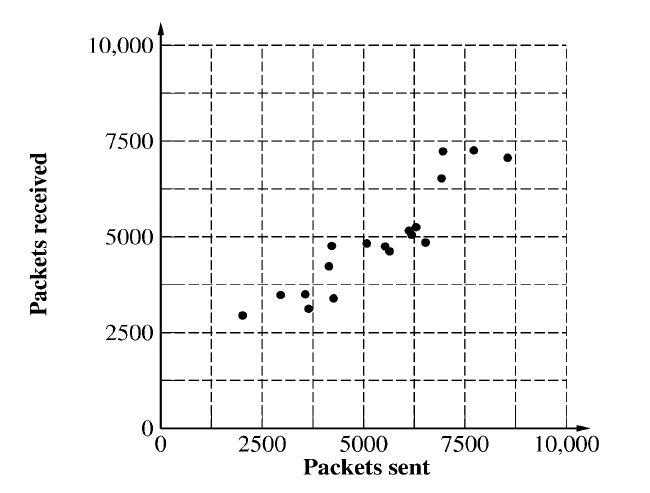
\includegraphics[width=\textwidth]{img/multi-histogram.png}
\caption{Multiparameter Histogram on 2D space}\label{img:multi-histogram}
\end{subfigure}

\hfill

\begin{subfigure}[b]{0.8\textwidth}
\centering
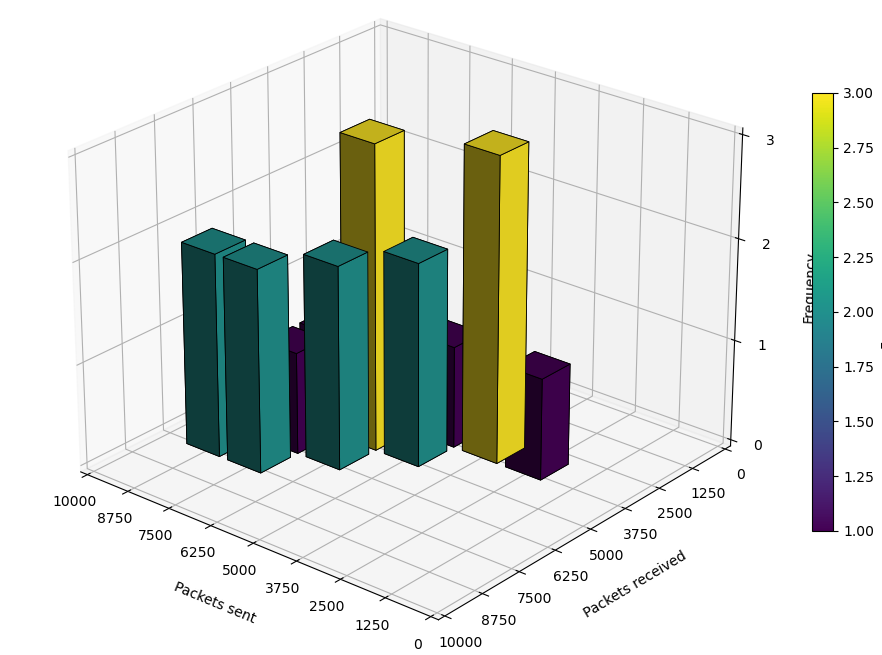
\includegraphics[width=.8\textwidth]{img/multi-histogram-3d.png}
\caption{Multiparameter Histogram on 3D space}
\label{img:multi-histogram-3d}
\end{subfigure}

\caption{Esempi di istogrammi multiparametrici}\label{fig:multi-histograms}
\end{figure}

\clearpage
\subsection{Principal Component Analysis (PCA)}
Un modo utilizzato per ridurre il numero di parametri con cui andare a rappresentare le istanze del workload è la \textbf{Principal Component Analysis (PCA)}. Tale tecnica ha come compito quello di trasformare l'insieme di istanze in altre istanze, le nuove istanze vengono definite sulla base delle componenti principali (che differiscono dai parametri reali), poichè nel nuovo spazio, tali parametri sono tutti linearmente indipendenti, e non ci sono correlazioni. Il funzionamento matematico della PCA è basato sull'effettuazione di una media pesata per ogni parametro. Precisamente:
\\
Dati i parametri \({x_1,x_2,\dots,x_N}\), si vuole trovare un nuovo insieme di parametri \({y_1,y_2,\dots,y_N}\), voglio però che l'insieme di parametri \(y_i\) sia linearmente indipendente, e che la varianza di ogni parametro \(y_i\) sia massimizzata. Di base per vedere come andare a costruire la matrice di trasformazione della PCA, si dovrebbe calcolare la matrice di covarianza, una volta calcolata si valutano gli autovettori di tale matrice, che costruiranno poi la matrice di trasformazione finale. Gli autovettori, quindi, rappresentano le direzioni principali e sono disposti in maniera che la prima componente principale sia quella con la varianza maggiore. Difatto si sta andando a fare una media pesata dei parametri per costruire il valore della nuova componente principale. Precisamente:
\[
y_j = \sum_{i=1}^{N}w_{ij}x_{ij}
\]

Tale formula va letta in questo modo:
\begin{itemize}
    \item \textbf{\(y_j\)}: rappresenta la j-esima componente principale
    \item \textbf{\(x_{ij}\)}: rappresenta il valore del parametro \(i\) nell'istanza \(j\)
    \item \textbf{\(w_{ij}\)}: rappresenta il peso associato al parametro \(i\) per la j-esima istanza
\end{itemize}

Per effettuare la PCA bisogna seguire i seguenti passi:
\begin{enumerate}
    \item Andare a calcolare la matrice di covarianza dei dati (prima si potrebbero effettuare anche operazioni di normalizzazione)
    \item Andare a calcolare gli autovettori e gli autovalori della matrice di covarianza
    \item Costruire la matrice di trasformazione mediante gli autovettori ordinati secondo gli autovalori in maniera decrescente (gli autovalori portano con loro la quantità di varianza, quindi ordinando gli autovettori si avrà uno spazio in cui il primo parametro copre la maggior varianza [utile per la selezione di un minor numero di parametri])
\end{enumerate}

In maniera più compatta, quindi, effettuata la PCA, si avrà che:
\begin{itemize}
    \item I nuovi parametri y sono calcolabili come combinazioni lineari dei parametri x
    \item I parametri y sono linearmente indipendenti, dato che il prodotto interno tra due parametri y è 0
    \item Il nuovo set di parametri y è ordinato in maniera tale che la varianza del primo parametro è maggiore della varianza del secondo e così via
\end{itemize}

\subsubsection{Z-Score Normalization}
La \textbf{z-score normalization} è una tecnica che permette di andare a normalizzare i dati, in maniera tale che ogni parametro abbia media 0 e deviazione standard 1. Tale tecnica è utile per poter effettuare la PCA, dato che si vuole evitare che parametri con range di valori molto diversi tra di loro possano influenzare in maniera sproporzionata il risultato finale. La formula per effettuare tale normalizzazione è la seguente:
\[
x'_s = \frac{x_{s} - \overline{x_s}}{s_{x_s}}
\]

Tale operazione permette di poter confrontare i parametri con un distribuzione normale, il che, quindi, andrà a rappresentare i dati come distanza da 0 e rappresentato secondo la deviazione standard s. Ciò ci permette anche di poter confrontare i dati tra di loro, senza andarea a considerare il range di valori che possono assumere.

\subsection{Clustering}
Mediante l'utilizzo della PCA si è andata ad effettuare la riduzione della quantità di parametri rappresentativi di un istanza (o componente) del workload. Per ridurre ancora di più la quantità di dati di rappresentazione del workload, si può andare ad effettuare una riduzione della quantità di istanze stesse. Per effettuare tale riduzione si fa utilizzo del \textbf{Clustering}, che è una tecnica di apprendimento non supervisionato che permette di andare a raggruppare le istanze in base alla loro similarità. Ciò richiede anche che la rappresentazione delle istanze sia adeguata per trovare degli specifici agglomerati di dati. (Per comprendere meglio, guardare la figura [\ref{img:clustering}], se i dati non fossero ben divisi non potrei creare i cluster per bene dato che avrei molta confusione)

\begin{figure}[h]
\centering
\includegraphics[width=.6\textwidth]{img/clustering.png}
\caption{Esempio di clustering}\label{img:clustering}
\end{figure}
